\renewcommand{\SourceFile}{4-arborescences/src/4-1.ml}

\section{Tas}

Un arbre binaire complet est un graphe comme celui de la figure : tous les niveaux sont remplis de gauche à droite, sauf éventuellement le dernier niveau. On numérote les sommets de 1 à $n$, niveau par niveau, et pour chaque niveau, de gauche à droite. S'il y a une flèche de $i$ vers $j$, on dit que $i$ est le père de $j$, et que $j$ est un fils de $i$. Le sommet d'en haut qui n'a pas de père (niveau 0), est la racine. Les sommets du dernier niveau, qui n'ont pas de fils, sont des feuilles. À chaque sommet numéro $i$, on associe un attribut entier. On représente alors un arbre binaire complet de taille $n$ par un tableau de taille $n+1$ dont la première case contient le nombre d'éléments du tas.
\medskip

\hspace{1cm}
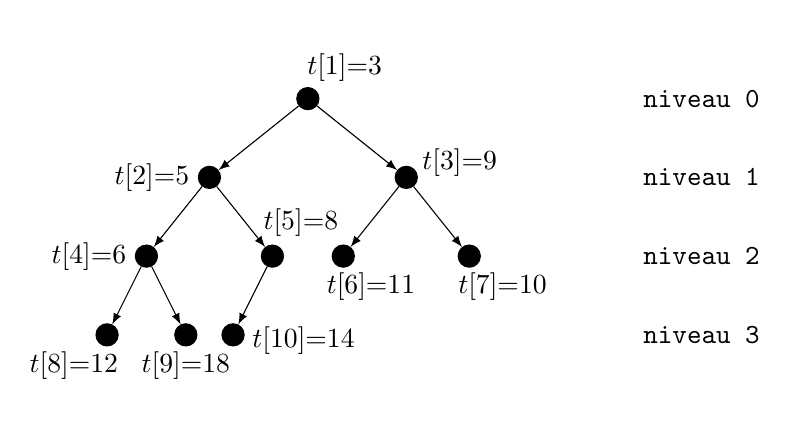
\begin{tikzpicture}
    [edge from parent/.style={draw,-latex},
    every node/.style={
        draw,
        fill=black,
        circle,
        inner sep=0pt,
        minimum size=8pt},
    level distance=1cm,
     level 1/.style={sibling distance=2.5cm},
     level 2/.style={sibling distance=1.6cm},
     level 3/.style={sibling distance=1cm}]
     \node[label={[yshift=-2pt]north east:$t\lbrack1\rbrack{=}3$}] {}
     child {node[label={[xshift=-2pt]left:$t\lbrack2\rbrack{=}5$}] {}
       child {node[label={[xshift=-2pt]left:$t\lbrack4\rbrack{=}6$}] {}
         child {node[label={[yshift=10pt, xshift=-12pt]south:$t\lbrack8\rbrack{=}12$}] {}}
         child {node[label={[yshift=10pt]south:$t\lbrack9\rbrack{=}18$}] {}}
       }
       child {node[label={[xshift=-3pt, yshift=-1pt]north east:$t\lbrack5\rbrack{=}8$}] {}
         child {node[label={[xshift=2pt, yshift=-2pt]right:$t\lbrack10\rbrack{=}14$}] {}}
         child[missing]
       }
     }
     child {node[label={[xshift=6pt, yshift=-8pt]north east:$t\lbrack3\rbrack{=}9$}] {}
       child {node[label={[yshift=10pt, xshift=10pt]south:$t\lbrack6\rbrack{=}11$}] {}}
       child {node[label={[yshift=10pt, xshift=12pt]south:$t\lbrack7\rbrack{=}10$}] {}}
     };
    \node[draw=none, fill=none] at (5, 0) {\texttt{niveau 0}};
    \node[draw=none, fill=none] at (5, -1) {\texttt{niveau 1}};
    \node[draw=none, fill=none] at (5, -2) {\texttt{niveau 2}};
    \node[draw=none, fill=none] at (5, -3) {\texttt{niveau 3}};
\end{tikzpicture}

\Q
Pour $i$ donné, $1 \leq i \leq n$, quel est son père, et quels sont ses fils (s'ils existent) ? Un tas est un arbre binaire complet dans lequel tout père est plus petit que ses fils (comme pour la figure). Le minimum est donc à la racine. Écrire une fonction OCaml qui vérifie si un arbre binaire complet est un tas.

\Q
Écrire une fonction OCaml qui supprime la racine d'un tas à $n$ sommets et qui renvoie un tas composé des $n-1$ sommets restants (indication : on pourra mettre la dernière feuille à la place de la racine et la faire descendre).

\Q
Comment insérer un nouvel élément dans un tas à $n$ sommets ?

\Corrige

\Q
Le père du sommet $i$ est $\lfloor i/2 \rfloor$ pour $2 \leq i \leq n$ (le père du sommet 1 n'est pas défini).
\smallskip

Les fils de $i$ sont $2i$ et $2i+1$ si ces valeurs sont $\leq n$. En particulier :
\begin{itemize}
    \item si $n$ est le nombre de sommets et $2i=n$, alors $i$ n'a qu'un fils, à savoir $n$
    \item si $i>\lfloor n/2 \rfloor$, alors $i$ est une feuille
\end{itemize}
Pour la fonction demandée, on vérifie les attributs des fils des sommets qui ne sont pas des feuilles, et on sort dès qu'il y a un échec :

\lstinputlisting[linerange={1-9}]{\SourceFile}

\Q
Une idée naturelle serait d'essayer de remonter le plus petit des fils de la racine à sa place, puis de continuer ainsi... mais on aboutit à un déséquilibre de l'arbre, qui n'est plus complet. Comme l'indication le suggère, il est plus simple de placer le dernier élément à la racine puis de le descendre à la bonne place (percolation basse) :

\lstinputlisting[linerange={11-35}]{\SourceFile}

La procédure a une complexité au pire proportionnelle au nombre de niveaux de l'arbre soit $\lceil \log_2n\rceil$.

\Q
Comme précédemment, une idée simple est d'ajouter la nouvelle valeur en dernière position, puis de la remonter tant que besoin est (percolation haute) :

\lstinputlisting[linerange={37-51}]{\SourceFile}

Ici encore, la fonction a une complexité proportionnelle au nombre de niveaux de l'arbre, donc en $O(\lceil \log_2n \rceil)$.
\medskip

Signalons que la structure de tas est à la base d'une méthode de tri très performante : le tri par tas. L'idée est simple : on part du tableau \texttt{a} de $n$ éléments à trier, et on construit un tas par ajout successif des $n$ éléments. On retire ensuite toutes les racines et on obtient ainsi les éléments dans l'ordre :

\lstinputlisting[firstline=53]{\SourceFile}

Le coût de chaque insertion ou suppression est proportionnel à la hauteur du tas courant ($\log_2p$ pour $p$ éléments), et donc le coût total est de l'ordre de :
\[
\sum_{p=1}^{n}\log_2p=\log_2n!=O(n\log_2n)
\]
(d'après la formule de Stirling ou par comparaison avec $\int_{1}^{n}\log x\,\mathrm{d}x$). Le tri par tas est donc asymptotiquement très rapide.
\bigskip

\Fin
